\documentclass{article}
\usepackage[utf8]{inputenc}
\usepackage{graphicx}

\title{CSE344 - HW1 Report}
\author{Abdullah Çelik}
\date{March 2021}

\begin{document}
\maketitle

\section{Overview}
\begin{itemize}
    \item The set$\_$arguments () function separates the command line arguments using the getopt() function. After doing this, the suitability of the parameters is tested (mentioned in the error handling section). In case of an error, the error message is returned. If everything goes well, NULL is returned. In this way, the user will be informed with an error message. Parameters are assigned to global variables in Srch$\_$Basis.h.
    \item The findByCriteria() function calls the function (find()) that will call the recursion. If there is an I / O error, -1 is returned and the error is printed in the screen with the perror() function. With Exit (1) the program is terminated.
    \item The find() function makes recursion calls and starts looking for the appropriate file in the given path. Creates a tree structure from the paths of the files it finds. If it cannot find the file it is looking for, the tree will not be created and a message will be printed on the screen.
    \item A path tree is created containing all the files found. This allows us to write the parent of every file found over and over again. It provides a more understandable output to the user. You can see the difference in the figure below.
\end{itemize}

\begin{figure}[h]
	\centering
	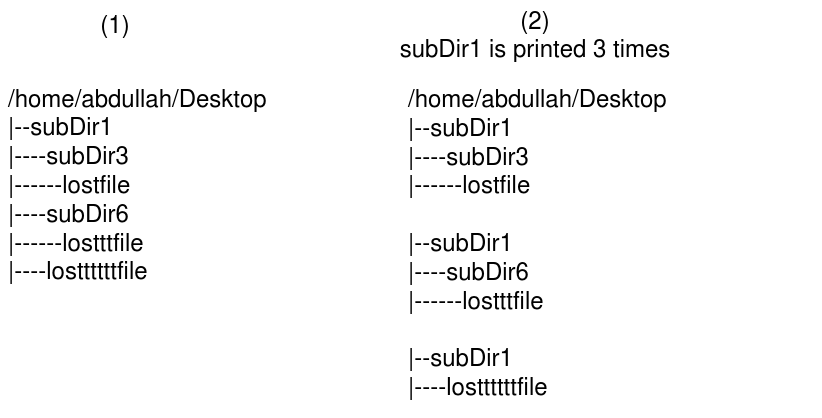
\includegraphics[scale=0.3]{fig1.png}
\end{figure}
\newpage

\section{Error Handling}

\begin{itemize}
\item CTRL + C
\newline
Description: The case where the user presses CTRL and C combination.
\newline
Action: Program gives all resources to memory and terminates itself.
\item The length of the given file name
\newline
Description: The case where the length of the file name given as a command line argument is greater than 255.
\newline
Action: "Error! The length of the file name cannot be greater than 255." message is printed to stderr and the program is terminated.
\item The type of given file size
\newline
Description: The case where the file size given as a command line argument is not integer.
\newline
Action: "Error! The file size must be integer." message is printed to stderr and the program is terminated.
\item Option of the file type
\newline
Description: The case where the file type given as a command line argument is invalid such as -t x.
\newline
Action: "Error! Wrong file type." message is printed to stderr and the program is terminated. 
\item The permissions parameter
\newline
Description: The case where the permissions gives as a command line argument is not 9 characters or it is invalid.
\newline
Action: "Error! Incorrect permission." message is printed to stderr and the program is terminated.
\item The type of number of links
\newline
Description: The case where the number of links given as a command line argument is not integer.
\newline
Action: "Error! Incorrect number of links." message is printed to stderr and program is terminated.
\item Not using any operator
\newline
Description: The case where the search criteria does not contain any combination of parameters.
\newline
Action: "Error! An operator must be used." message is printed to stderr and program is terminated.
\item Not using -w parameter
\newline
Description: The case where the mandatory path parameter does not received.
\newline
Action: "Error! The -w parameter is mandatory." message is printed to stderr and program is terminated.
\item Using undefined operation
\newline
Description: The case where the undefined operation is used such as -x.
\newline
Action: "Error! Undefined operation." message is printed to stderr and program is terminated.
\item Using additional parameters
\newline
Description: The case where the additional parameter is used such as -f file additionalParameter.
\newline
Action: "Error! Additional parameter is founded." message is printed and program is terminated.
\item Incorrect use of regexp
\newline
Description: The case where the file name contains a regexp in the first character.
\newline
Action: "Error! Incorrect usage of regexp." message is printed to stderr and program is terminated.
\item Using opendir function
\newline
Description: The case where the opendir function returns NULL (this means an error is occurred) after calling (inside of findByCriteria function).
\newline
Action: If the value returned by the opendir is checked and an error occurs, the error is printed with the perror function and the program is terminated with exit(1).
\item Using readdir function
\newline
Description: The case where the readdir function returns NULL (The readdir function return NULL in two cases. First case is If the end of the directory stream is reached, NULL is returned and errno is not changed. The second case if If an error occurs, NULL is returned an errno is set appropriately.) after calling (inside of findByCriteria function).
\newline
Action: Before calling readdir function, errno is saved. Then after calling readdir function, it is checked whether errno is change or not. If there is a change, error is printed with perror function and program is terminated with exit(1).
\item Using lstat function
\newline
Description: The case where the lstat function returns -1 (this means an error is occurred) after calling (inside of findByCriteria function).
\newline
Action: If the value returned by the lstat is checked and an error occurs, the error is printed with the perror function and the program is terminated with exit(1).
\item Using closedir function
\newline
Description: The case where the closedir function returns -1 (this means an error is occurred) after calling (inside of findByCriteria function).
\newline
Action: If the value returned by the closedir is checked and an error occurs, the error is printed with the perror function and the program is terminated with exit(1).
\end{itemize}

\section{Compile and Run}

\begin{itemize}
    \item make $\rightarrow$ Compiles the whole program
    \newline
    Type make in the file contains the Makefile
    \item make clean $\rightarrow$ Cleans all objects files
\end{itemize}

\section{Testing}

The file structure is as follows.
\begin{figure*}[h]
	\centering
	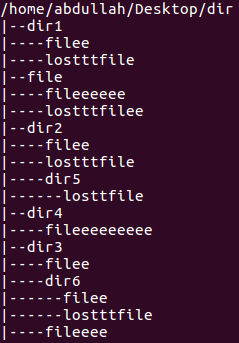
\includegraphics[scale=0.5]{t1.png}
\end{figure*}

./myFind -w /home/abdullah/Desktop/dir1/ -f file+
\begin{figure*}[h]
	\centering
	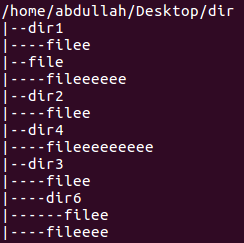
\includegraphics[scale=0.5]{t2.png}
\end{figure*}

\newpage
./myFind -w /home/abdullah/Desktop/dir -f lost+file
\begin{figure*}[h]
	\centering
	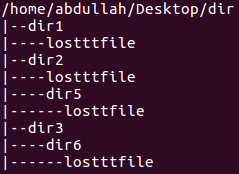
\includegraphics[scale=0.5]{t3.png}
\end{figure*}

./myFind -w /home/abdullah/Desktop/dir -t d
\begin{figure*}[h]
	\centering
	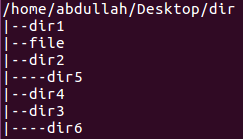
\includegraphics[scale=0.5]{t4.png}
\end{figure*}

./myFind -w /home/abdullah/Desktop/dir -f file+ -b 0 -t f -p rw-rw-r-- -l 1
\begin{figure*}[h]
	\centering
	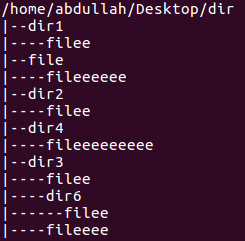
\includegraphics[scale=0.5]{t5.png}
\end{figure*}

\end{document}